\section{String\_\-Hash\_\-Value  Class Reference}
\label{classString__Hash__Value}\index{String_Hash_Value@{String\_\-Hash\_\-Value}}
{\tt \#include $<$string\_\-hash\_\-value.hh$>$}

Inheritance diagram for String\_\-Hash\_\-Value::\begin{figure}[H]
\begin{center}
\leavevmode
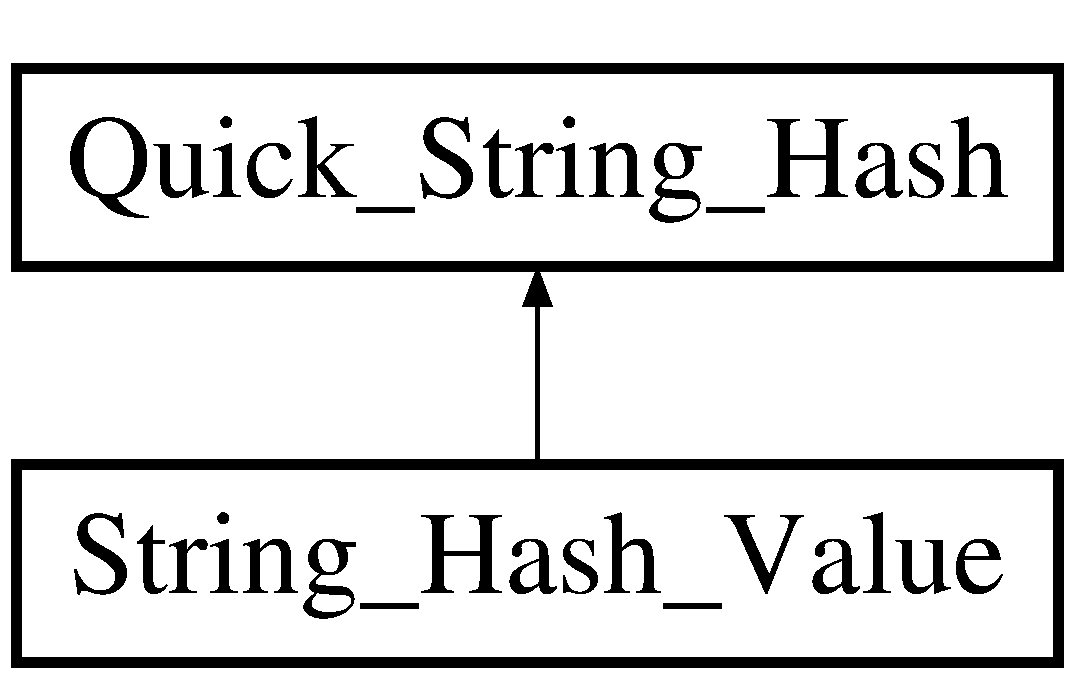
\includegraphics[height=2cm]{classString__Hash__Value}
\end{center}
\end{figure}
\subsection*{Public Methods}
\begin{CompactItemize}
\item 
{\bf String\_\-Hash\_\-Value} ()
\item 
String\_\-Hash\_\-Value \& {\bf insert\_\-value} (const char $\ast$s, int v)
\item 
int {\bf read\_\-value} (const char $\ast$s) const
\end{CompactItemize}
\subsection*{Protected Attributes}
\begin{CompactItemize}
\item 
int {\bf val}
\end{CompactItemize}


\subsection{Constructor \& Destructor Documentation}
\index{String_Hash_Value@{String\_\-Hash\_\-Value}!String_Hash_Value@{String\_\-Hash\_\-Value}}
\index{String_Hash_Value@{String\_\-Hash\_\-Value}!String_Hash_Value@{String\_\-Hash\_\-Value}}
\subsubsection{\setlength{\rightskip}{0pt plus 5cm}String\_\-Hash\_\-Value::String\_\-Hash\_\-Value ()\hspace{0.3cm}{\tt  [inline]}}\label{classString__Hash__Value_a0}




Definition at line 13 of file string\_\-hash\_\-value.hh.

References val.



\footnotesize\begin{verbatim}13 : Quick_String_Hash(), val(0) {}
\end{verbatim}\normalsize 


\subsection{Member Function Documentation}
\index{String_Hash_Value@{String\_\-Hash\_\-Value}!insert_value@{insert\_\-value}}
\index{insert_value@{insert\_\-value}!String_Hash_Value@{String\_\-Hash\_\-Value}}
\subsubsection{\setlength{\rightskip}{0pt plus 5cm}String\_\-Hash\_\-Value \& String\_\-Hash\_\-Value::insert\_\-value (const char $\ast$ {\em s}, int {\em v})}\label{classString__Hash__Value_a1}




Definition at line 21 of file string\_\-hash\_\-value.hh.

References Quick\_\-String\_\-Hash::add\_\-list\_\-element(), Quick\_\-String\_\-Hash::insert(), Quick\_\-String\_\-Hash::len, Quick\_\-String\_\-Hash::list, Quick\_\-String\_\-Hash::offset, and val.



\footnotesize\begin{verbatim}21                                                                          {
22         if (s[0]=='\0') {
23                 val = v;
24                 return (*this);
25         }
26         int i = ((int) s[0]);   // implied list coordinate
27         int r = i - offset;             // real list coordinate
28         if (r<0) {
29                 if (add_list_element(i)==NULL) return (*this);
30                 r = i - offset; // adjust to new offset
31         } else if (r>=len) {
32                 if (add_list_element(i)==NULL) return (*this); // this also takes care of the case where the list is unallocated
33                 r = i - offset; // adjust to new offset
34         } else if (!list[r]) {
35                 if (add_list_element(i)==NULL) return (*this);
36         }
37         list[r]->insert(&s[1]);
38         return (*this);
39 }
\end{verbatim}\normalsize 
\index{String_Hash_Value@{String\_\-Hash\_\-Value}!read_value@{read\_\-value}}
\index{read_value@{read\_\-value}!String_Hash_Value@{String\_\-Hash\_\-Value}}
\subsubsection{\setlength{\rightskip}{0pt plus 5cm}int String\_\-Hash\_\-Value::read\_\-value (const char $\ast$ {\em s}) const}\label{classString__Hash__Value_a2}




Definition at line 41 of file string\_\-hash\_\-value.hh.

References Quick\_\-String\_\-Hash::len, Quick\_\-String\_\-Hash::list, Quick\_\-String\_\-Hash::offset, and val.



\footnotesize\begin{verbatim}41                                                       {
42         int i; const String_Hash_Value * qsh = this;
43         for (const char * c = s; (*c!='\0'); c++) {
44                 i = ((int) *c); // implied list coordinate
45                 if (i<qsh->offset) return 0;
46                 i -= qsh->offset;       // real list coordinate
47                 if (i>=qsh->len) return 0; // this also takes care of the case where the list is unallocated
48                 if (!qsh->list[i]) return 0;
49                 qsh = qsh->list[i];     // traverse tree
50         }
51         return qsh->val;
52 }
\end{verbatim}\normalsize 


\subsection{Member Data Documentation}
\index{String_Hash_Value@{String\_\-Hash\_\-Value}!val@{val}}
\index{val@{val}!String_Hash_Value@{String\_\-Hash\_\-Value}}
\subsubsection{\setlength{\rightskip}{0pt plus 5cm}int String\_\-Hash\_\-Value::val\hspace{0.3cm}{\tt  [protected]}}\label{classString__Hash__Value_n0}




Definition at line 10 of file string\_\-hash\_\-value.hh.

Referenced by insert\_\-value(), read\_\-value(), and String\_\-Hash\_\-Value().

The documentation for this class was generated from the following file:\begin{CompactItemize}
\item 
{\bf string\_\-hash\_\-value.hh}\end{CompactItemize}
